\chapter{Causal Discovery}
Up till now, we have assumed that the causal structure of the data is known. However,
in many cases, the causal structure is not known and must be inferred from the data.
This is the problem of \textbf{causal discovery}.

\section{Causal Discovery from Observational Data}
Let's start by saying that learning a causal network consists of learning the
structure and the parameters of the network.
\subsection{Constraint-Based Methods}
We assume that the underlying process follows a probability distribution $P$, which
is the underlying probability distribution associated with a DAG $\mathcal{G}$.
Then, this process can be adequately described by sampling from $P$ to obtain
Observational Data.

The goal of constraint-based methods is to infer the structure of the DAG $\mathcal{G}$
from the observational data. To simplify the task, we assume the probability
distribution $P$ to be a DAG-faithful probability distribution with underlying
DAG $\mathcal{G}$.

The \textbf{faithfulness} assumption says that the probability distribution $P$,
induced by the DAG $\mathcal{G}$, satisfies no independence relations beyond
those implied by the DAG $\mathcal{G}$.

\begin{definition}[\textbf{Stability - faithfulness}]
    $P$ is a stable (faithful) distribution if there exists a DAG $\mathcal{G}$
    such that:
    \begin{equation}
        \mathbf{X} \perp_{P} \mathbf{Y} \mid \mathbf{Z} \quad \iff \quad \mathbf{X} \perp_{\mathcal{G}} \mathbf{Y} \mid \mathbf{Z}
    \end{equation}
    for any three sets of variables $\mathbf{X}$, $\mathbf{Y}$, and $\mathbf{Z}$.
\end{definition}

A causal network is \textbf{faithful} if and only if for every d-connection (no
d-separation) $\mathbf{Z}$ there is a corresponding conditional dependence:
\begin{equation}
    \mathbf{X} \not\perp_{\mathcal{G}} \mathbf{Y} \mid \mathbf{Z} \quad \Rightarrow \quad \mathbf{X} \not\perp_{P} \mathbf{Y} \mid \mathbf{Z}
\end{equation}

It is worthwhile to mention that many constraint-based methods also assume that there
are no unobserved confounders. This is known as the \textbf{Causal Sufficiency}
assumption.

Learning a causal network is the task of identifying a DAG structure $\mathcal{G}$
and a set of conditional probability distributions $\mathcal{P}$ with parameters
$\theta$ based on:
\begin{itemize}
    \item $\mathcal{D} = \{x^1, \ldots, x^N\}$ this are the observational data,
          where the missing data are assumed to be missing at random or missing
          completely at random.
    \item Possibly some domain expert knowledge.
\end{itemize}

A variable never observed is called a \textbf{latent variable}.

Structured learning is then the task of identifying a DAG structure that encodes
a set of dependence and independence relations $M_{\mathcal{G}}$, which may be
derived from observational data by statistical test.

A constraint-based structure learning algorithm proceeds by determining the validity
of independence relations of the form:
\begin{equation}
    I(X, Y| S_{XY})
\end{equation}
where $X$ is independent of $Y$ given $S_{XY}$.

The problem with this approach is that the number of possible independent relations
is exponential in the number of variables. In particular, a constraint-based
structure learning algorithm discovers a DAG structure of $P$ under the following
assumptions:
\begin{itemize}
    \item The independence relationships have a perfect representation as a DAG
          (Acyclicity and faithfulness assumptions);
    \item No hidden (latent) variables are involved (Causal Sufficiency assumption);
    \item The database (Observational Data) consists of a set of independent and
          identically distributed cases.
    \item The database (Observational Data) is infinitely large;
    \item The statistical tests have no error.
\end{itemize}

The equivalence class of a DAG $\mathcal{G}$ is the set of all DAGs with the same
set of d-separation relations as $\mathcal{G}$. The equivalence class can be represented
by a partially directed acyclic graph (PDAG).

\begin{definition}[\textbf{Equivalent Models And Markov equivalence Class}]
    Two models $M_\mathcal{G'}$ and $M_\mathcal{G''}$ defined over the same set
    of variables, whose graphs $\mathcal{G'}$ and $\mathcal{G''}$, respectively,
    have the same \textbf{skeleton} (i.e., the undirected graph obtained by replacing
    directed edges with undirected edges) and the same v-structures, are \textbf{equivalent}.

    Two graphs $\mathcal{G'}$ and $\mathcal{G''}$ are in the same \textbf{equivalence class}:
    \begin{itemize}
        \item if they share a common skeleton — that is, if they possess the same
              edges, regardless of the direction of those edges—and;
        \item if they share a common v-structure, that is, colliders whose parents
              are not adjacent
    \end{itemize}
\end{definition}

Given a graph, we refer to its Markov equivalence class as a set of graphs that
encode the same set of conditional independence relations.

\begin{definition}[\textbf{Equivalence Class}]
    An equivalence class is a maximal set of DAGs with the same set of independence
    properties $\mathcal{M}_{\mathcal{G}}$.
\end{definition}

A set of dependence and independence relations $M_{\mathcal{G}}$ may be generated
by statistical tests on the observational data. In each test, the hypothesis is
that of independence between a pair of variables.

Let $X$ and $Y$ be two variables for which we would like to determine dependence
by statistical hypothesis testing. We could:
\begin{itemize}
    \item test for marginal independence and subsequently;
    \item test for conditional independence given subsets of other variables.
\end{itemize}
\section{The PC algorithm}
The main steps of the PC algorithm are:
\begin{enumerate}
    \item Test for (conditional) independence between each pair of variables
          represented in $\mathcal{D} = \{x^1, \dots, x^N\}$ to derive $M_\mathcal{D}$,
          the set of conditional independence and dependence relations;
    \item Identify the skeleton of the graph induced by $M_\mathcal{D}$. For each
          pair of variables $X$ and $Y$ where no independence statement $X \perp_{P} Y | S_{XY}$
          exists, the undirected edge $X - Y$ is added to the skeleton;
    \item Identify colliders. Based on the skeleton, we search for subsets of variables $\{X, Y, Z\}$
          such that $X$ and $Y$ are neighbors, $Z$ and $Y$ are neighbors, and
          $X$ and $Z$ are not neighbors;
    \item Identify derived directions. The direction of an edge is said to be
          derived when it is a logical consequence of previous actions:
          \begin{itemize}
              \item \textbf{Rule 1}: since the edge between $Y$ and $Z$ is not part
                    of the aforementioned collider, it must be oriented as $Y \rightarrow Z$;
              \item \textbf{Rule 2}: directing an edge between $X$ and $Z$ from $Z$
                    to $X$ will induce a directed cycle in the graph.
              \item \textbf{Rule 3}: directing the edge between $X$ and $Y$ from
                    $Y$ to $X$ will induce an additional collider.
              \item \textbf{Rule 4}: directing the edge between $X$ and $Y$ from
                    $Y$ to $X$ will induce an additional collider.
          \end{itemize}
\end{enumerate}

The PC algorithm typically produces a PDAG (Partially DAG) representing an equivalence
class as it emerges from hypothesis testing performed by using the available
observational data $\mathcal{D} = \{x^1, \dots, x^N\}$.

\section{Semi-parametric Causal Discovery}
\begin{definition}[\textbf{Markov Completeness}]
    If we have multinomial distribution or linear Gaussian structural equations,
    we can only identify a graph up to its Markov equivalence class.
\end{definition}

We now introduce and study two cases where we can identify the causal graph. And
we don't have to assume faithfulness in these settings:
\begin{itemize}
    \item non-Gaussian noise setting;
    \item non-linear additive noise setting.
\end{itemize}
By considering these settings, we are making a semi-parametric assumption. If we
don't make any assumptions about functional form, we cannot even identify the
direction of the edge in a two-node graph.
\begin{definition}[\textbf{Non-Identidiability of two-node graphs}]
    For every joint distribution $P(X, Y)$ on two real-valued random variables,
    there is a SCM in either direction that generates data consistent with $P(X, Y)$.

    Mathematically, there exists a function $f_Y$ such that:
    \begin{equation*}
        Y := f_Y(X, U_Y) \quad X \perp U_Y
    \end{equation*}
    and there exists a function $f_X$ such that:
    \begin{equation*}
        X := f_X(Y, U_X) \quad Y \perp U_X
    \end{equation*}
    where $U_X$ and $U_Y$ are real-valued random variables.
\end{definition}
This non-identifiability result can be extended to more general graphs that have
more than two variables. However, if we make assumptions about the parametric form
of the SCM, we can distinguish the graphs and identify graphs more generally.

An example of these assumptions is the following:
\begin{definition}[\textbf{Linear Non-Gaussian}]
    All structural equations (the causal mechanisms that generate the data) are
    of the following form:
    \begin{equation}
        Y := f(X) + U
    \end{equation}
    where $f$ is a linear function, $X \perp U$, and $U$ is distributed as a 
    non-Gaussian random variable.
\end{definition}

\begin{definition}[\textbf{identifiability in Linear Non-Gaussian Setting}]
    In the linear non-Gaussian setting, if the true SCM is:
    \begin{equation*}
        Y := f(X) + U \quad X \perp U
    \end{equation*}
    then, there does not exist an SCM in the reverse direction:
    \begin{equation*}
        X := f(Y) + \tilde{U} \quad Y \perp \tilde{U}
    \end{equation*}
    that can generate data consistent with $P(X, Y)$.
\end{definition}

\begin{theorem}[\textbf{Darmois-Skitovich Theorem}]
    Let $X_1, \dots, X_n$ be independent, nondegenerate random variables. If there
    exists coefficients $\alpha_1, \dots, \alpha_n$ and $\beta_1, \dots, \beta_n$ such that:
    \begin{equation*}
        \begin{split}
            A = \alpha_1X_1 + \dots + \alpha_nX_n \\
            B = \beta_1X_1 + \dots + \beta_nX_n
        \end{split}
    \end{equation*}
    are independent, then each $X_i$ is normally distributed.
\end{theorem}
\begin{corollary}[\textbf{Darmois-Skitovich Corollary}]
    If either of the independent random variables $X_1$ or $X_2$ is non-Gaussian,
    then there are no linear combinations:
    \begin{equation}
        \begin{split}
            A = \alpha_1X_1 + \alpha_2X_2 \\
            B = \beta_1X_1 + \beta_2X_2
        \end{split}
    \end{equation}
    such that $A$ and $B$ are independent (so $A$ and $B$ must be dependent).
\end{corollary}
We can also get the identifiability of the causal graph in the \textbf{non-linear additive
    noise setting}. This requires a nonlinear additive noise assumption:
\begin{definition}[\textbf{Non-Linear Additive Noise}]
    All causal mmechanismsare non-linear where the noise enters additively.
    Mathematically:
    \begin{equation}
        \forall i, X_i := f_i(Pa(X_i)) + U_i
    \end{equation}
    where $f$ is non-linear and $pa(X_i)$ are the parents of $X_i$ in the graph.
\end{definition}
We could also have that the noise does not enter additively, but this is a more
complicated setting.
\begin{definition}[\textbf{Post Non-Linear}]
    \begin{equation}
        \forall i, X_i := g(f(pa(X_i)) + U_i)
    \end{equation}
    where $f$ is a non-linear function and $pa(X_i)$ are the parents of $X_i$ in
    the graph.
\end{definition}
\section{Additional Topics}
Structural learning of Bayesian (causal) networks consists of three approaches:
\begin{itemize}
    \item \textbf{Constraint-Based algorithm}: they use statistical tests to learn
          conditional independence relationships (called “constraints" in this
          setting) from the data by making specific assumptions to determine the
          correct network structure. They depend heavily on the quality of the
          conditional independence tests they use; all proofs of correctness
          assume tests are always right.
    \item \textbf{Score-Based algorithm}: each candidate DAG is assigned a score
          reflecting its goodness of fit, which is then taken as an objective
          function to maximize. Convergence to the global maximum (i.e. the best
          structure) is not guaranteed for finite samples, the search may get
          stuck in a local maximum.
    \item \textbf{Hybrid algorithm}: conditional independence tests are used to
          learn at least part of the conditional independence relationships from
          the data, thus restricting the search space for a subsequent score-based
          Search. The latter determines which edges are present in the
          graph and their direction.
\end{itemize}
\section{Causal Discovery from Interventional Data}
Let's start by defining the types of interventions:
\begin{itemize}
    \item \textbf{Perfect}: interventions are represented by the do-operator;
    \item \textbf{Imperfect}: interventions alter the parameters of the network.
\end{itemize}
\subsection{Single-Node interventions}
The simplest case is the two-variable case, i.e. the bi-variate setting, where
either: $X$ is cause of $Y$, or $Y$ is cause of $X$, or $X$ is not cause of $Y$,
and $Y$ is not cause of $Y$.

To identify the graph two interventions are necessary and sufficient,
dividing the empty set case from a proper interventional set setting.

\begin{figure}[!ht]
    \centering
    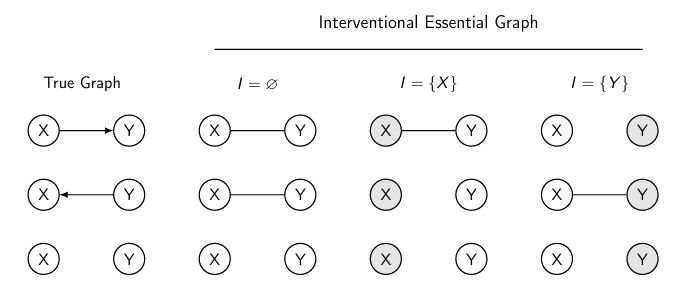
\includegraphics[width=\textwidth]{img/causal_discovery/twonodecase.png}
    \caption{Two-node case}
    \label{fig:twonodecase}
\end{figure}

In the worst-case scenario, $n- 1$ interventions are sufficient:
\begin{enumerate}
    \item Choose an arbitrary intervention ordering;
    \item Applying the first intervention identifies the adjacencies of the $n - 1$
          nodes;
    \item Applying the $i$-th intervention directs the edges incident on $X_i$,
    \item Applying the $n$-th intervention is unnecessary, since the remaining
          directions are identified in the $(n-1)$-th step.
\end{enumerate}
In the worst case, $n-1$ interventions are necessary:
\begin{enumerate}
    \item Choose an arbitrary intervention ordering;
    \item Applying the $(n-2)$-th interventions leaves the $X_{n - 1} - X_n$ edge
          undirected;
    \item Applying the $(n-1)$-th intervention is necessary to direct the last
          edge.
\end{enumerate}
Therefore, $n-1$ interventions are necessary and sufficient in the worst case
scenario (given $n > 2$)
\subsection{Multi-Node Interventions}
If we apply multi/nodes interventions, with no restrictions on the nodes a
$\lfloor \log_2(n) \rfloor + 1$ interventions are necessary and sufficient to
identify the graph.

If we start from the Markov equivalence class a $\lceil \log_2(c) \rceil$ are
necessary and sufficient, with $c$ the size of the largest clique.